\documentclass[tikz,border=2pt]{standalone}
\usepackage{amsmath}
\usetikzlibrary{arrows.meta}
\begin{document}
% In R^3, W = span{(1,1,1)^T} is a line and W^perp = {x_1 + x_2 + x_3 = 0} is the plane through 0
% perpendicular to it, spanned by (-1,1,0)^T and (-1,0,1)^T (both of length sqrt 2, at 60 degrees);
% drawn with an orthonormal frame of the plane plus the unit normal, so lengths and angles in the plane are true.
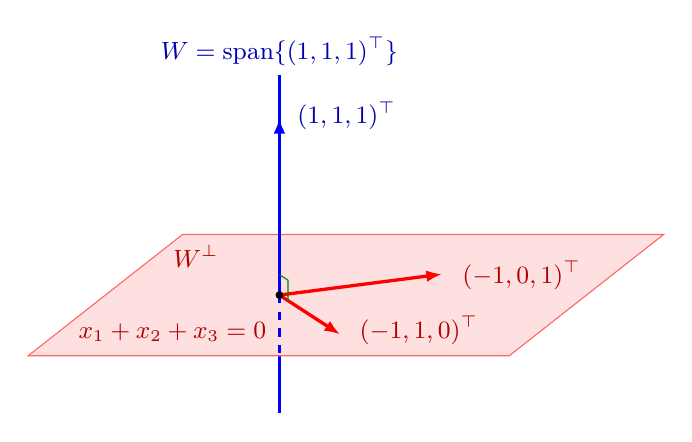
\begin{tikzpicture}[font=\small, >={Latex[length=2mm]}, x={(1.3cm,0cm)}, y={(0.7cm,0.55cm)}, z={(0cm,1.3cm)}]
  % hidden part of the line below the plane, then the visible part below the front edge
  \draw[blue, thick] (0,0,-0.592) -- (0,0,-1.15);
  % the plane W^perp
  \fill[red!12] (-1.7,-1.4,0) -- (3.0,-1.4,0) -- (3.0,1.4,0) -- (-1.7,1.4,0) -- cycle;
  \draw[red!60] (-1.7,-1.4,0) -- (3.0,-1.4,0) -- (3.0,1.4,0) -- (-1.7,1.4,0) -- cycle;
  \draw[blue, thick, dashed] (0,0,0) -- (0,0,-0.592);
  % spanning vectors of W^perp: (-1,1,0)^T at -40 deg and (-1,0,1)^T at +20 deg in the plane frame
  \draw[->, red, very thick] (0,0,0) -- (1.0834,-0.9091,0);
  \node[red!70!black, anchor=west] at (1.13,-0.82,0) {$(-1,1,0)^{\top}$};
  \draw[->, red, very thick] (0,0,0) -- (1.3289,0.4837,0);
  \node[red!70!black, anchor=west] at (1.45,0.45,0) {$(-1,0,1)^{\top}$};
  \node[red!70!black] at (-1.3,0.9,0) {$W^\perp$};
  \node[red!70!black, anchor=west] at (-1.6,-0.85,0) {$x_1+x_2+x_3=0$};
  % the line W and its spanning vector (length sqrt 3)
  \draw[blue, thick] (0,0,0) -- (0,0,2.15);
  \draw[->, blue, very thick] (0,0,0) -- (0,0,1.7321);
  \node[blue!70!black, anchor=west] at (0.08,0,1.75) {$(1,1,1)^{\top}$};
  \node[blue!70!black, anchor=south] at (0,0,2.15) {$W=\operatorname{span}\{(1,1,1)^{\top}\}$};
  % right angle between W and the plane
  \draw[green!50!black] (0,0,0.2) -- (0.1532,-0.1286,0.2) -- (0.1532,-0.1286,0);
  \fill (0,0,0) circle (1.4pt);
\end{tikzpicture}
\end{document}
